%% bare_conf.tex
%% V1.4
%% 2012/12/27
%% by Michael Shell
%% See:
%% http://www.michaelshell.org/
%% for current contact information.
%%
%% This is a skeleton file demonstrating the use of IEEEtran.cls
%% (requires IEEEtran.cls version 1.8 or later) with an IEEE conference paper.
%%
%% Support sites:
%% http://www.michaelshell.org/tex/ieeetran/
%% http://www.ctan.org/tex-archive/macros/latex/contrib/IEEEtran/
%% and
%% http://www.ieee.org/

%%*************************************************************************
%% Legal Notice:
%% This code is offered as-is without any warranty either expressed or
%% implied; without even the implied warranty of MERCHANTABILITY or
%% FITNESS FOR A PARTICULAR PURPOSE! 
%% User assumes all risk.
%% In no event shall IEEE or any contributor to this code be liable for
%% any damages or losses, including, but not limited to, incidental,
%% consequential, or any other damages, resulting from the use or misuse
%% of any information contained here.
%%
%% All comments are the opinions of their respective authors and are not
%% necessarily endorsed by the IEEE.
%%
%% This work is distributed under the LaTeX Project Public License (LPPL)
%% ( http://www.latex-project.org/ ) version 1.3, and may be freely used,
%% distributed and modified. A copy of the LPPL, version 1.3, is included
%% in the base LaTeX documentation of all distributions of LaTeX released
%% 2003/12/01 or later.
%% Retain all contribution notices and credits.
%% ** Modified files should be clearly indicated as such, including  **
%% ** renaming them and changing author support contact information. **
%%
%% File list of work: IEEEtran.cls, IEEEtran_HOWTO.pdf, bare_adv.tex,
%%                    bare_conf.tex, bare_jrnl.tex, bare_jrnl_compsoc.tex,
%%                    bare_jrnl_transmag.tex
%%*************************************************************************

% *** Authors should verify (and, if needed, correct) their LaTeX system  ***
% *** with the testflow diagnostic prior to trusting their LaTeX platform ***
% *** with production work. IEEE's font choices can trigger bugs that do  ***
% *** not appear when using other class files.                            ***
% The testflow support page is at:
% http://www.michaelshell.org/tex/testflow/


% Note that the a4paper option is mainly intended so that authors in
% countries using A4 can easily print to A4 and see how their papers will
% look in print - the typesetting of the document will not typically be
% affected with changes in paper size (but the bottom and side margins will).
% Use the testflow package mentioned above to verify correct handling of
% both paper sizes by the user's LaTeX system.
%
% Also note that the "draftcls" or "draftclsnofoot", not "draft", option
% should be used if it is desired that the figures are to be displayed in
% draft mode.
%
\documentclass[conference]{IEEEtran}
\usepackage[utf8]{inputenc}
\usepackage[norsk]{babel}
\usepackage{csquotes} % For å legge på språkspesifikke anførselstegn. I teksten brukes \enquote{text}
%\usepackage{hyperref}
\usepackage{varioref}
\usepackage{listings} % For å importere kode
\usepackage{xcolor} % For å legge farge på koden

\definecolor{codegreen}{rgb}{0,0.6,0}
\definecolor{codegray}{rgb}{0.5,0.5,0.5}
\definecolor{codepurple}{rgb}{0.58,0,0.82}
\definecolor{codered}{rgb}{0.53,0,0.08}
\definecolor{backcolour}{rgb}{0.95,0.95,0.92}

\lstdefinestyle{mystyle}{
    backgroundcolor = \color{backcolour},   
    commentstyle = \color{codegreen},
    keywordstyle = \color{codepurple},
    keywordstyle = [2]{\color{orange}},
    numberstyle = \tiny\color{codegray},
    stringstyle = \color{codered},
    basicstyle = \ttfamily\footnotesize,
    breakatwhitespace = false,         
    breaklines = true,                 
    captionpos = b,                    
    keepspaces = true,                 
    numbers = left,                    
    numbersep = 5pt,                  
    showspaces = false,                
    showstringspaces = false,
    showtabs = false,                  
    tabsize = 2
}
\lstdefinestyle{rapid}{
    backgroundcolor = \color{backcolour},   
    commentstyle = \color{codegreen},
    morecomment = [l][commentstyle]{!},
    keywordstyle = \color{blue},
    keywordstyle = [2]{\color{teal}},
    keywords = {MODULE,PROC,WHILE,IF,THEN,DO,OR,ELSE,ELSEIF,ENDIF,ENDWHILE,ENDPROC,ENDMODULE, VAR, CONST, RAISE, RETRY},
    morekeywords = [2]{MoveL, MoveJ, Offs, StrLen, StrPart, StrToVal, SocketAccept, SocketBind, SocketClose, SocketConnect, SocketCreate, SocketListen, SocketReceive, SocketSend, TPWrite, WaitTime, robtarget, num, socketdev, string, ERRNO, ERR_SOCK_CLOSED, ERR_SOCK_TIMEOUT, fine , v100, v1000},
    numberstyle = \tiny\color{codegray},
    stringstyle = \color{codered},
    morestring = [b][stringstyle]",
    basicstyle = \ttfamily\footnotesize,
    breakatwhitespace = false,         
    breaklines = true,                 
    captionpos = b,                    
    keepspaces = true,                 
    numbers = left,                    
    numbersep = 5pt,                  
    showspaces = false,                
    showstringspaces = false,
    showtabs = false,                  
    tabsize = 2
}

\lstset{style=mystyle}


% Add the compsoc option for Computer Society conferences.
%
% If IEEEtran.cls has not been installed into the LaTeX system files,
% manually specify the path to it like:
% \documentclass[conference]{../sty/IEEEtran}





% Some very useful LaTeX packages include:
% (uncomment the ones you want to load)


% *** MISC UTILITY PACKAGES ***
%
%\usepackage{ifpdf}
% Heiko Oberdiek's ifpdf.sty is very useful if you need conditional
% compilation based on whether the output is pdf or dvi.
% usage:
% \ifpdf
%   % pdf code
% \else
%   % dvi code
% \fi
% The latest version of ifpdf.sty can be obtained from:
% http://www.ctan.org/tex-archive/macros/latex/contrib/oberdiek/
% Also, note that IEEEtran.cls V1.7 and later provides a builtin
% \ifCLASSINFOpdf conditional that works the same way.
% When switching from latex to pdflatex and vice-versa, the compiler may
% have to be run twice to clear warning/error messages.






% *** CITATION PACKAGES ***
%
%\usepackage{cite}
% cite.sty was written by Donald Arseneau
% V1.6 and later of IEEEtran pre-defines the format of the cite.sty package
% \cite{} output to follow that of IEEE. Loading the cite package will
% result in citation numbers being automatically sorted and properly
% "compressed/ranged". e.g., [1], [9], [2], [7], [5], [6] without using
% cite.sty will become [1], [2], [5]--[7], [9] using cite.sty. cite.sty's
% \cite will automatically add leading space, if needed. Use cite.sty's
% noadjust option (cite.sty V3.8 and later) if you want to turn this off
% such as if a citation ever needs to be enclosed in parenthesis.
% cite.sty is already installed on most LaTeX systems. Be sure and use
% version 4.0 (2003-05-27) and later if using hyperref.sty. cite.sty does
% not currently provide for hyperlinked citations.
% The latest version can be obtained at:
% http://www.ctan.org/tex-archive/macros/latex/contrib/cite/
% The documentation is contained in the cite.sty file itself.






% *** GRAPHICS RELATED PACKAGES ***
%
\ifCLASSINFOpdf
  \usepackage{graphicx}
  \usepackage{tikz}
  \usetikzlibrary{quotes,angles}
  % declare the path(s) where your graphic files are
  % \graphicspath{{../pdf/}{../jpeg/}}
  % and their extensions so you won't have to specify these with
  % every instance of \includegraphics
  % \DeclareGraphicsExtensions{.pdf,.jpeg,.png}
\else
  % or other class option (dvipsone, dvipdf, if not using dvips). graphicx
  % will default to the driver specified in the system graphics.cfg if no
  % driver is specified.
  % \usepackage[dvips]{graphicx}
  % declare the path(s) where your graphic files are
  % \graphicspath{{../eps/}}
  % and their extensions so you won't have to specify these with
  % every instance of \includegraphics
  % \DeclareGraphicsExtensions{.eps}
\fi
% graphicx was written by David Carlisle and Sebastian Rahtz. It is
% required if you want graphics, photos, etc. graphicx.sty is already
% installed on most LaTeX systems. The latest version and documentation
% can be obtained at: 
% http://www.ctan.org/tex-archive/macros/latex/required/graphics/
% Another good source of documentation is "Using Imported Graphics in
% LaTeX2e" by Keith Reckdahl which can be found at:
% http://www.ctan.org/tex-archive/info/epslatex/
%
% latex, and pdflatex in dvi mode, support graphics in encapsulated
% postscript (.eps) format. pdflatex in pdf mode supports graphics
% in .pdf, .jpeg, .png and .mps (metapost) formats. Users should ensure
% that all non-photo figures use a vector format (.eps, .pdf, .mps) and
% not a bitmapped formats (.jpeg, .png). IEEE frowns on bitmapped formats
% which can result in "jaggedy"/blurry rendering of lines and letters as
% well as large increases in file sizes.
%
% You can find documentation about the pdfTeX application at:
% http://www.tug.org/applications/pdftex





% *** MATH PACKAGES ***
%
\usepackage[cmex10]{amsmath}
% A popular package from the American Mathematical Society that provides
% many useful and powerful commands for dealing with mathematics. If using
% it, be sure to load this package with the cmex10 option to ensure that
% only type 1 fonts will utilized at all point sizes. Without this option,
% it is possible that some math symbols, particularly those within
% footnotes, will be rendered in bitmap form which will result in a
% document that can not be IEEE Xplore compliant!
%
% Also, note that the amsmath package sets \interdisplaylinepenalty to 10000
% thus preventing page breaks from occurring within multiline equations. Use:
%\interdisplaylinepenalty=2500
% after loading amsmath to restore such page breaks as IEEEtran.cls normally
% does. amsmath.sty is already installed on most LaTeX systems. The latest
% version and documentation can be obtained at:
% http://www.ctan.org/tex-archive/macros/latex/required/amslatex/math/





% *** SPECIALIZED LIST PACKAGES ***
%
%\usepackage{algorithmic}
% algorithmic.sty was written by Peter Williams and Rogerio Brito.
% This package provides an algorithmic environment fo describing algorithms.
% You can use the algorithmic environment in-text or within a figure
% environment to provide for a floating algorithm. Do NOT use the algorithm
% floating environment provided by algorithm.sty (by the same authors) or
% algorithm2e.sty (by Christophe Fiorio) as IEEE does not use dedicated
% algorithm float types and packages that provide these will not provide
% correct IEEE style captions. The latest version and documentation of
% algorithmic.sty can be obtained at:
% http://www.ctan.org/tex-archive/macros/latex/contrib/algorithms/
% There is also a support site at:
% http://algorithms.berlios.de/index.html
% Also of interest may be the (relatively newer and more customizable)
% algorithmicx.sty package by Szasz Janos:
% http://www.ctan.org/tex-archive/macros/latex/contrib/algorithmicx/




% *** ALIGNMENT PACKAGES ***
%
%\usepackage{array}
% Frank Mittelbach's and David Carlisle's array.sty patches and improves
% the standard LaTeX2e array and tabular environments to provide better
% appearance and additional user controls. As the default LaTeX2e table
% generation code is lacking to the point of almost being broken with
% respect to the quality of the end results, all users are strongly
% advised to use an enhanced (at the very least that provided by array.sty)
% set of table tools. array.sty is already installed on most systems. The
% latest version and documentation can be obtained at:
% http://www.ctan.org/tex-archive/macros/latex/required/tools/


% IEEEtran contains the IEEEeqnarray family of commands that can be used to
% generate multiline equations as well as matrices, tables, etc., of high
% quality.




% *** SUBFIGURE PACKAGES ***
\ifCLASSOPTIONcompsoc
  \usepackage[caption=false,font=normalsize,labelfont=sf,textfont=sf]{subfig}
\else
  \usepackage[caption=false,font=footnotesize]{subfig}
\fi
% subfig.sty, written by Steven Douglas Cochran, is the modern replacement
% for subfigure.sty, the latter of which is no longer maintained and is
% incompatible with some LaTeX packages including fixltx2e. However,
% subfig.sty requires and automatically loads Axel Sommerfeldt's caption.sty
% which will override IEEEtran.cls' handling of captions and this will result
% in non-IEEE style figure/table captions. To prevent this problem, be sure
% and invoke subfig.sty's "caption=false" package option (available since
% subfig.sty version 1.3, 2005/06/28) as this is will preserve IEEEtran.cls
% handling of captions.
% Note that the Computer Society format requires a larger sans serif font
% than the serif footnote size font used in traditional IEEE formatting
% and thus the need to invoke different subfig.sty package options depending
% on whether compsoc mode has been enabled.
%
% The latest version and documentation of subfig.sty can be obtained at:
% http://www.ctan.org/tex-archive/macros/latex/contrib/subfig/




% *** FLOAT PACKAGES ***
%
%\usepackage{fixltx2e}
% fixltx2e, the successor to the earlier fix2col.sty, was written by
% Frank Mittelbach and David Carlisle. This package corrects a few problems
% in the LaTeX2e kernel, the most notable of which is that in current
% LaTeX2e releases, the ordering of single and double column floats is not
% guaranteed to be preserved. Thus, an unpatched LaTeX2e can allow a
% single column figure to be placed prior to an earlier double column
% figure. The latest version and documentation can be found at:
% http://www.ctan.org/tex-archive/macros/latex/base/


%\usepackage{stfloats}
% stfloats.sty was written by Sigitas Tolusis. This package gives LaTeX2e
% the ability to do double column floats at the bottom of the page as well
% as the top. (e.g., "\begin{figure*}[!b]" is not normally possible in
% LaTeX2e). It also provides a command:
%\fnbelowfloat
% to enable the placement of footnotes below bottom floats (the standard
% LaTeX2e kernel puts them above bottom floats). This is an invasive package
% which rewrites many portions of the LaTeX2e float routines. It may not work
% with other packages that modify the LaTeX2e float routines. The latest
% version and documentation can be obtained at:
% http://www.ctan.org/tex-archive/macros/latex/contrib/sttools/
% Do not use the stfloats baselinefloat ability as IEEE does not allow
% \baselineskip to stretch. Authors submitting work to the IEEE should note
% that IEEE rarely uses double column equations and that authors should try
% to avoid such use. Do not be tempted to use the cuted.sty or midfloat.sty
% packages (also by Sigitas Tolusis) as IEEE does not format its papers in
% such ways.
% Do not attempt to use stfloats with fixltx2e as they are incompatible.
% Instead, use Morten Hogholm'a dblfloatfix which combines the features
% of both fixltx2e and stfloats:
%
% \usepackage{dblfloatfix}
% The latest version can be found at:
% http://www.ctan.org/tex-archive/macros/latex/contrib/dblfloatfix/




% *** PDF, URL AND HYPERLINK PACKAGES ***
%
\usepackage{url}
% url.sty was written by Donald Arseneau. It provides better support for
% handling and breaking URLs. url.sty is already installed on most LaTeX
% systems. The latest version and documentation can be obtained at:
% http://www.ctan.org/tex-archive/macros/latex/contrib/url/
% Basically, \url{my_url_here}.




% *** Do not adjust lengths that control margins, column widths, etc. ***
% *** Do not use packages that alter fonts (such as pslatex).         ***
% There should be no need to do such things with IEEEtran.cls V1.6 and later.
% (Unless specifically asked to do so by the journal or conference you plan
% to submit to, of course. )


% correct bad hyphenation here
\hyphenation{op-tical net-works semi-conduc-tor}
\addto{\captionsnorsk}{\renewcommand{\abstractname}{Sammendrag}}
\usepackage{multicol}
\begin{document}
%
% paper title
% can use linebreaks \\ within to get better formatting as desired
% Do not put math or special symbols in the title.
\title{Objektgjenkjenning og sortering med robotarm}

% author names and affiliations
% use a multiple column layout for up to three different
% affiliations
% |-- En forfatterblokk --|
\author{\IEEEauthorblockN{Kenneth R. Eikrehagen $\cdot$ Lars-Erik Ulvund, \\ Alexsander Kristensen $\cdot$ Erik Johansson}
\IEEEauthorblockA{\textit{Institutt for maskin, elektronikk og kjemi} \\ OsloMet – storbyuniversitetet \\ Oslo, Norge\\ s331475@oslomet.no $\cdot$ s331432@oslomet.no \\ s331477@oslomet.no $\cdot$ s330317@oslomet.no} \\ 7. desember 2020}

% conference papers do not typically use \thanks and this command
% is locked out in conference mode. If really needed, such as for
% the acknowledgment of grants, issue a \IEEEoverridecommandlockouts
% after \documentclass

% use for special paper notices
%\IEEEspecialpapernotice{(Invited Paper)}




% make the title area
\maketitle

% As a general rule, do not put math, special symbols or citations
% in the abstract
\begin{abstract}
    Denne prosjektoppgaven inneholder nesten to prosjekter da roboten som ble brukt til første prosjektet ble ødelagt etter to uker. 
    Gruppen ble godt kjent med NAO sitt brukergrensesnitt gjennom dens egne programmeringsverktøy \textit{Choreographe} og Aldebran sitt 
    naoqi-bibliotek i Python 2.7. NAO roboten ble programmert til å finne og gå mot en rød ball før den ble ødelagt. 

    I det endelige prosjektet er det brukt en industriell robotarm fra ABB og objekgjenkjenning. 
    Det ble utarbeidet en løsning som sorterer geometriske figurer etter fasong. For å få til dette 
    er det benyttet Python programmering med bruk av \textit{OpenCV} som henter video fra et kamera som er 
    festet i taket over robotarmen. Socket programming er brukt som kommunikasjonsledd mellom Python 
    og RobotStudio til å sende informasjon om figurtype og dens posisjon. Dette gjorde det mulig for 
    robotarmen å plukke opp den riktige figuren og sortere den til korrekt endestasjon. 
\end{abstract}

% no keywords




% For peer review papers, you can put extra information on the cover
% page as needed:
% \ifCLASSOPTIONpeerreview
% \begin{center} \bfseries EDICS Category: 3-BBND \end{center}
% \fi
%
% For peerreview papers, this IEEEtran command inserts a page break and
% creates the second title. It will be ignored for other modes.
\IEEEpeerreviewmaketitle



\section{Introduksjon}
% no \IEEEPARstart
Dette prosjektet har blitt inspirert av hvordan kunstig intelligens (KI), tingenes internett (IoT) og skytjenester har påvirket robotteknikk, 
samt hvordan dette kan fortsette å påvirke denne industrien. På leting etter et prosjekt som kunne passe til dette stakk NAO roboten som hører
til i laboratoriet for Automatisering, Robotikk og Intelligente Systemer (ARIS-lab) seg frem som et godt utgangspunkt. NAO er konstruert for å 
skape forståelse om hvordan KI kan brukes i sammenheng med robotteknikk der internett blir brukt som kommunikasjonskanal. To uker inn i prosjektet 
ble NAO-roboten ødelagt og prosjektplanen måtte endres. 

Kjerneideen fra ovennevnte prosjekt ble tatt med videre inn i nytt prosjekt. Dette ved bruk av kombinasjonen KI og robotteknikk med kommunikasjon 
gjennom et Internett Protokoll nettverk (IP-nettverk). Det ble vurdert at en god måte å implementere dette var ved å kombinere et kamera, socket 
programmering over Transmission Control Protocol  (TCP) og en industriell robotarm fra ABB.

    \subsection{NAO prosjekt}
    I dette prosjektet skulle NAO roboten undersøke synsfeltet sitt etter en ball. Deretter gå bort til ballen for så å plukke den opp og kaste den. 
    Det var også ønskelig at NAO roboten skulle respondere på stemmekommando. 
\newpage
        Prosjektets tre utfordringer:
        \begin{enumerate}
            \item Detektere en ball deretter gå bort til den 
            \item Plukke opp ballen og kaste den
            \item Reagere på stemmekommando 
        \end{enumerate}
        
        Dessverre ble roboten ødelagt to uker inn i prosjektperioden. På dette tidspunktet var første utfordring unnagjort, 
        og en løsning til neste steg var under utarbeidelse. Mye tid gikk med for å finne kilder til hvordan å kunne programmere roboten med Python 2.7 
        og brukergrensesnittet til Python-NAO-biblioteket (naoqi). Biblioteket naoqi hadde mange gode funksjoner som kunne brukes i prosjektet, med 
        større fokus på robotteknikk enn KI algoritmer. Koden som ble produsert under dette prosjektet finner man i Tillegg seksjon A.

    \subsection{ABB prosjekt}
        ABB-robotarmen på ARIS-lab ble utrustet med et sugekopp-verktøy, og det er montert et kamera rett over robotarmen. Problemstillingen å bruke 
        objektgjenkjenning sammen med robotarmen til å sortere forskjellige geometriske figurer ble raskt unnfanget. De viktigste utfordringene identifisert 
        med dette prosjektet var:
        \begin{enumerate}
            \item Finne en måte å bruke dataen fra kameraet i taket
            \item Detektere og finne forskjellige geometriske figurer
            \item Få robotarmen til å bevege seg til riktig figur
        \end{enumerate}
        Videre undersøkelser viste at den beste løsningen var å bruke Python 3.8 (heretter referert til som Python) sammen med OpenCV-biblioteket til å 
        anvende kameraet i taket for objektgjenkjenning. Programvaremessig er Python og RobotStudio brukt for å bevege robotarm ved bruk av socket programmering 
        som kommunikasjonsledd. De geometriske figurene som ble brukt for å teste algoritmen var trekant, firkant, sekskant og sirkel.

\section{Teori}

    \subsection{NAO robot}
        Aldebaran Robotics har laget en liten \textit{humanoid robot} kalt NAO som er designet for å samhandle med mennesker. Denne kan gå, danse og snakke. I tillegg 
        kan den gjenkjenne ansikt, stemmer og objekter. Denne roboten har nå kommet til sjette generasjon og blir brukt i undervisning, forskning og helsevesen \cite{teori:NAO}. 
        Den har 25 grader av frihet, syv berøringssensorer, fire retningsbestemte mikrofoner og høyttalere, stemmegjenkjenning, to 2D kameraer og en åpen 
        og fullt programmerbar plattform \cite{teori:SBNAO}.

    \subsection{Objektgjenkjenning}
        Objektgjenkjenning er en datateknologi som benytter datasyn og bildebehandling for å oppdage objekter av en bestemt klasse, f.eks. mennesker, biler eller sykler i digitale bilder og videoer. For å gjenkjenne objekter benyttes det maskinlæring. 

        \subsubsection{Maskinlæring}
            Prosessen med å bruke matematiske datamodeller til å hjelpe en datamaskin med å lære uten direkte instruksjon kalles maskinlæring (ML) \cite{teori:ML}. 
            Dette kan være en enklere tilnærming som baserer seg på forhåndsdefinerte egenskaper eller kjennetegn som sier noe om hva det letes etter 
            og hvordan det skal finnes, hvor dataen etterpå blir klassifisert ved å bruke f.eks. Support Vector Machine (SVM).

    \subsection{OpenCV}
    Et programvarebibliotek som ofte blir brukt for konstruksjon av kildekode for maskinlæring og datamaskinsyn er OpenCV.  Biblioteket er utviklet for å tilby en felles infrastruktur for datasynapplikasjoner og for å akselerere bruken av maskinoppfattelse i kommersielle produkter. OpenCV sitt grensesnitt inkluderer C++, Python, Java og MATLAB og inneholder over 2500 algoritmer innenfor maskinlæring og datasyn \cite{teori:OpenCV}. 

    \subsection{ABB-robotarm}
        ABB-robotarm IRB 140 er en relativ liten, men kraftig robotarm som jobber med seks akser. Robotarmen har en rekkevidde på 810mm til 
        akse fem og en løftekapasitet på maks seks kg. Det finnes nesten ingen begrensninger for hvor mange forskjellige verktøy som kan monteres 
        på enden av robotarmen, deriblant en sugekopp. Basen til robotarmen kan monteres enten til bakken/underlaget, i taket eller til veggen, 
        noe som gjør robotarmen veldig allsidig \cite{teori:ABB}. 

    \subsubsection{Robotstudio}
        Robotarmen styres av programmer som er laget i ABB sitt program RobotStudio. Programmet overføres til en såkalt FlexPendant, som er 
        koblet til og styrer robotarmen. RobotStudio har en innebygget funksjon som gjør det mulig å simulere ønsket program før det testes 
        på den fysiske roboten.

        I RobotStudio er det mulig å modellere gjenstander, figurer og workobjects. En løsning som gjør at simuleringer i programmet enkelt kan 
        gjenspeile virkeligheten. Selve programmet skrives i RAPID, et programmeringsspråk utviklet for ABB sine industrielle roboter. 
        Programmet bygges opp av flere moduler for å oppnå god struktur. RAPID har en rekke interne biblioteker og funksjoner som gjør prosessen 
        med å konstruere forskjellige programmer relativ enkel \cite{teori:RobStud} \cite{teori:RobStud1}. 

    \subsection{Socket programmering}
        Socket kommunikasjon brukes for å få to noder i et nettverk til å kommunisere med hverandre ved hjelp av meldinger eller pakker.Det kan være 
        et logisk og internt nettverk i en datamaskin. Alternativt et som er fysisk tilkoblet et åpent ytre nettverk. Det er mulig å sende og motta 
        slike meldinger nesten hvor som helst så lenge man har en internettforbindelse \cite{teori:socket}.

        Nodene defineres som tjener og klient hvor den ene noden (tjeneren) lytter på en bestemt port mens den andre (klienten) søkes ut for å etablere 
        en tilkobling.

        Kommunikasjonsprotokollen som normalt brukes er TCP, hvor man har god kontroll på at meldingene mottas i den formen de ble sendt. Mottakeren 
        kan bekrefte meldingen og pakker som ikke når frem overføres på nytt av avsender, dette blir godt illustrert på figur \ref{fig:socket}.
        \begin{figure}
            \centering
            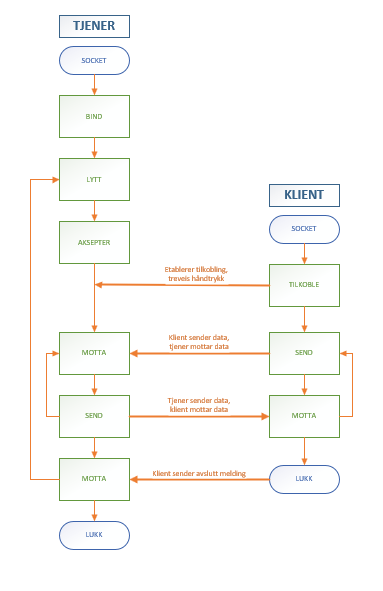
\includegraphics[width=.8\linewidth]{images/socket_flytskjema.png}
            \caption{Flytskjema som viser hvordan socket programmering med TCP fungerer}
            \label{fig:socket}
        \end{figure}
        \subsubsection{Transport Control Protocol (TCP)}
            Både tjener og klient etablerer socket. Tjeneren binder socketen til spesifisert adresse og port, og lytter passivt etter klientens 
            forsøk på tilkobling. Når tjeneren aksepterer en innkommende forespørsel om tilkobling gjøres et treveis håndtrykk for å bekrefte at 
            kommunikasjonen er etablert. Meldinger kan så sendes fritt mellom nodene. Klientens socket lukkes ofte etter utført operasjon, slik at 
            tjeneren kan gå tilbake til passiv lyttemodus, men dette avhenger litt av hensikt og applikasjon.
    
\section{Metode}
    \begin{figure}
        \centering
        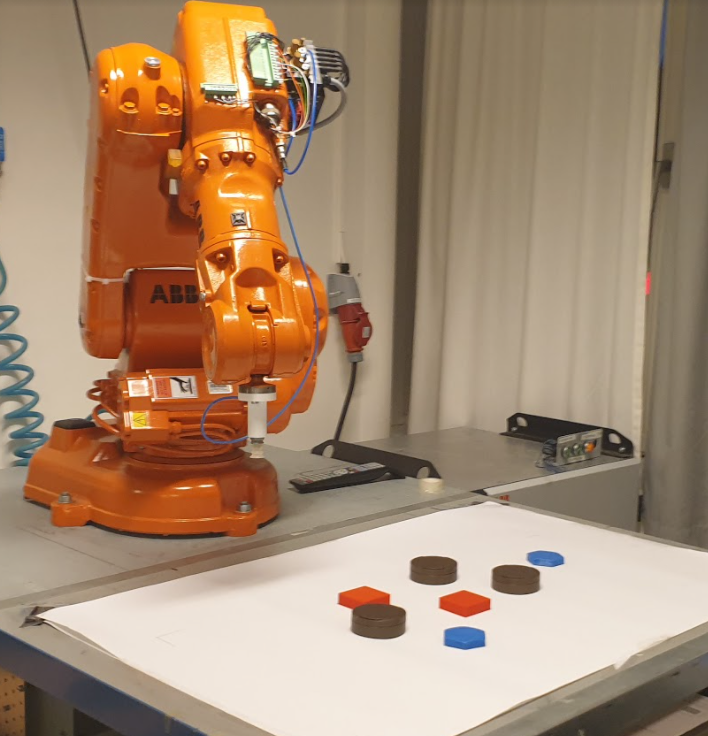
\includegraphics[width=.8\linewidth]{images/robotarm.png}
        \caption{Robotarmen som ble brukt sammen med figurene den skulle sortere}
        \label{fig:metode}
    \end{figure}

    I denne prosjektoppgaven er objektgjenkjenning sammen med ABB-robotarmen brukt til å sortere forskjellige geometriske figurer som vist på figur \ref{fig:metode} på neste side. OpenCV og  Python-programmering er benyttet for gjennomføring av objektgjenkjenning. ABB-robotarm med sugekopp-verktøy er anvendt for den fysiske sorteringen av figurene. Hvordan robotarmen skulle oppføre seg ble programmert gjennom RAPID i RobotStudio. For å etablere kommunikasjon mellom Python og RobotStudio over internett måtte det benyttes socket programmering.

    Algoritmen som ble konstruert ble testet med at robotarmen skulle sortere fire forskjellige geometriske figurer. Figurene som skulle sorteres var trekant, firkant, sirkel og sekskant. For enkelheten sin skyld ble benevnelsen forkortet til respektive TRI, SQR, CRC og HEX for videre kommunikasjon 
    med robotarmen. 
    
    For utstyrsliste se tillegg seksjon B tabell \ref{app:soft} og \ref{app:hard}. 
    
    \subsection{ABB-robotarm}
        Til å sortere de ulike geometriske figurene er det benyttet en ABB-robotarm. Programmet som kjøres på FlexPendant er skrevet i RAPID. 
        
        Robotarmen ble utstyrt med et sugekopp-verktøy som flyttet de forskjellige figurene fra synsfeltet til kameraet og over til en predefinert endestasjon. 

        For å verifisere arbeidsområdet til robotarmen ble det plassert et hvit ark på bordet foran robotarmen. Kameraet i taket ble skrudd på og prosjektert på en pc-skjerm.
        
        En firkantet figur ble plassert i hvert av hjørnene i henhold til hva kameraet kunne detektere og hjørnene ble markert på det hvite arket.

    \subsection{Objektgjenkjenning}
        OpenCV ble brukt sammen med Python for å kunne fange og prosessere video av ønsket arbeidsområde. For å kommunisere med kamera i taket var det også nødvendig å installere en ekstern driver \cite{metode:kamera}, ettersom kameraet ikke var \textit{plug-and-play}.

        Det som kjennetegner en geometrisk figur er hvor mange kanter den har. OpenCV har en funksjon som kan detektere antall kanter til objekter i bildet. Dette kalles \textit{edge detection} og er en gren som tilhører objektgjenkjenning. Denne funksjonen utførte først objektlokalisering for å finne figurene, deretter ble det telt opp hvor mange kanter figurene hadde.
        
        Antall kanter ble så analysert for å kjenne igjen hvilke typer geometriske figurer den så på bildet. Ut ifra dette kunne man også kalkulere senterpunktet til hver figur. De foreløpige verdiene måtte deretter skaleres fra piksel-dimensjon til metriske verdier. Dette ble gjort ved å beregne forholdet mellom høyden i bildet med tilsvarende høyde på arbeidsområdet.
        
        I forbindelse med videre kommunikasjon til robotarmen var det nødvendig å etablere et referansepunkt.  Det viste seg at OpenCV analyserte bildet som en matrise ved at den startet i det øverste venstre hjørnet, og jobbet seg bortover rad for rad. Referansen for videre kommunikasjon måtte derfor være øverst til venstre i bildet.
        % # TODO: Dele opp i flere avsnitt?

    \subsection{Socket programmering}
        For å oppnå kommunikasjon mellom Python koden som tok seg av objektgjenkjenningen og RobotStudio som beveger robotarmen ble det benyttet socket programmering. Python programmet ble satt opp til å være en klient, og robotarmen ble konfigurert til å være server. Før dataen kunne sendes videre til robotarmen måtte alle numeriske verdier konverteres til datatypen \textit{string}.  Dette ble gjort i en egendefinert funksjon som tok i mot antall identifiserte kanter, samt piksel koordinater til senter i figurene og returnerte dette som en string. Beskjeden som ble sendt inneholdt benevnelsen av hvilken type figur samt senter koordinatene til figuren.

    \subsection{RobotStudio}
        For at ABB-robotarmen skulle plukke opp figurene var det viktig å synkronisere arbeidsområdet til kameraet med arbeidsområdet til robotarmen. 
        Kameraet var montert slik at på videoen som ble vist var hjørnet oppe til venstre for kameraet tilsvarende hjørnet nede til høyre for basen til robotarmen. Programmet som ble laget i Python sendte koordinater med utgangspunkt fra hjørnet oppe til venstre. Der X-aksen strakk seg langs øvre kant og Y-aksen nedover langs bildets venstre kant.

       \begin{figure}[!htb]
            \centering
                \includegraphics[width=.8\linewidth]{images/Arbeidsområde.png}
            \caption{Arbeidsområde definert i forhold til bildeutsnitt brukt i OpenCV}
            \label{fig:robotstudio}
        \end{figure}

        Løsningen som ble valgt var å lage et workobject i RobotStudio som tilsvarer arbeidsområdet til kameraet som vist i figur \ref{fig:robotstudio}. Arbeidsområdets vinkel i forhold til arbeidsbordet ble justert ved hjelp av en trigonometrisk funksjon:
        \begin{equation*}
            \text{Vinkel } \alpha = tan^{-1}\frac{a}{b}
        \end{equation*}
        og er vist i figur \ref{fig:trig}

        \begin{figure}[!htb]
            \centering
            \begin{tikzpicture}
                % \draw[style=help lines] (0,0) grid (3,2);
                \filldraw[fill=orange!20!white, draw=orange] (0,0) -- (0,2.5) arc (90:85:2.5) node[orange,above right=-1pt]{$\alpha$} -- (0,0);
                \draw[gray] (0,0) -- node[left] {b} (0,10/3) node[above right=-2.5pt] {a} -- (5,10/3) -- (5,0) -- (0,0);
                \draw[rotate around={-5:(0,0)}] (0,0) -- node[right] {c} (0,10/3) -- (5,10/3) -- (5,0) -- (0,0);
            \end{tikzpicture}
            \caption{Hvordan man finner vinkel $\alpha$ mellom to plan}
            \label{fig:trig}
        \end{figure}
    
        Siden kameraet er montert i taket oppfatter den figurene kun i 2D. Det vil si at kameraet ikke kan detektere høydene på figurene som vises i arbeidsområdet. Høyden på de forskjellige figurene må derfor pre defineres for hver figur. 

        For å unngå at de sorterte geometriske figurene ikke skulle forveksles som figurer som skulle sorteres ble endestasjonene satt til å være utenfor synsfeltet til kameraet.

    \subsection{Figurene}
        For å vise at prosjektet med objektgjenkjenning kunne kjenne igjen forskjellige geometriske figurer falt valget ned på fire forskjellig figurer. Hver med forskjellig høyde. En trekant med en høyde på 20 mm, firkant med høyde 15 mm, sekskant med høyde 10 mm og sirkel med høyde 24 mm. 
        De geometriske figurene firkant, trekant og sekskant ble tegnet i Tinkercad \cite{metode:tinkercad} og 3D-printet med bruk av PLA. PLA er et termoplastisk materiale som er relativt lufttett. Dette gjør det lettere for sugekopp-verktøyet til robotarmen å plukke opp de geometriske figurene. Sirkelen som er benyttet er en gammel snusboks som er laget av plast. PLA ble valgt fordi det var gratis og tilgjengelig på MakerSpace.

        
\section{Resultater}
    Prosjektet ble en suksess. Robotarmen klarte å sortere objektene som vist i figur \ref{resultat:robotarm}. 
    Figur \ref{resultat:sortering} illustrerer hvordan robotarmen sorterer objektene som er tilfeldig plassert i arbeidsområdet.
    \begin{figure}[!htb]
        \centering
        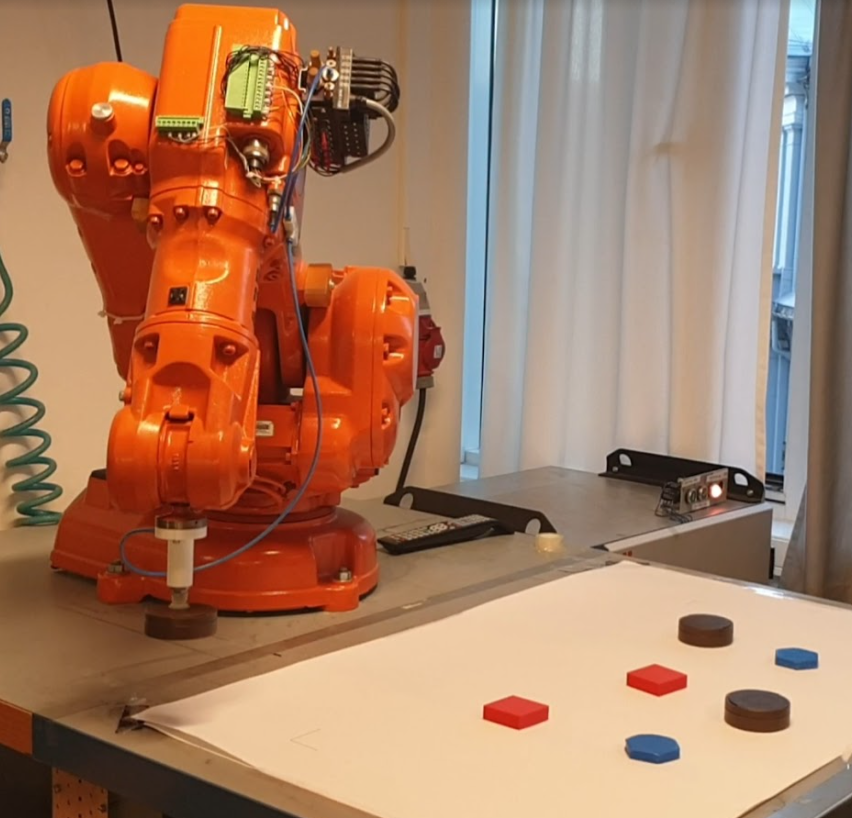
\includegraphics[width=.8\linewidth]{images/robotarm1.png}
        \caption{Her er et bilde av robotarmen som starter å sortere objektene}
        \label{resultat:robotarm}
    \end{figure}

    \begin{figure}
        \centering
        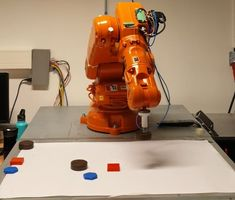
\includegraphics[width = .8\linewidth]{images/sortering.jpg}
        \caption{Her ser man at robotarmen har sortert objektene til venste, og de resterende objektene i arbeidsområdet er tilfeldig plassert}
        \label{resultat:sortering}
    \end{figure}

    Kantdeteksjon med kamera og OpenCV fugerte godt. Resultatet er vist i figur \ref{resulat:objekt}.
    \begin{figure}[!htb]
        \centering
        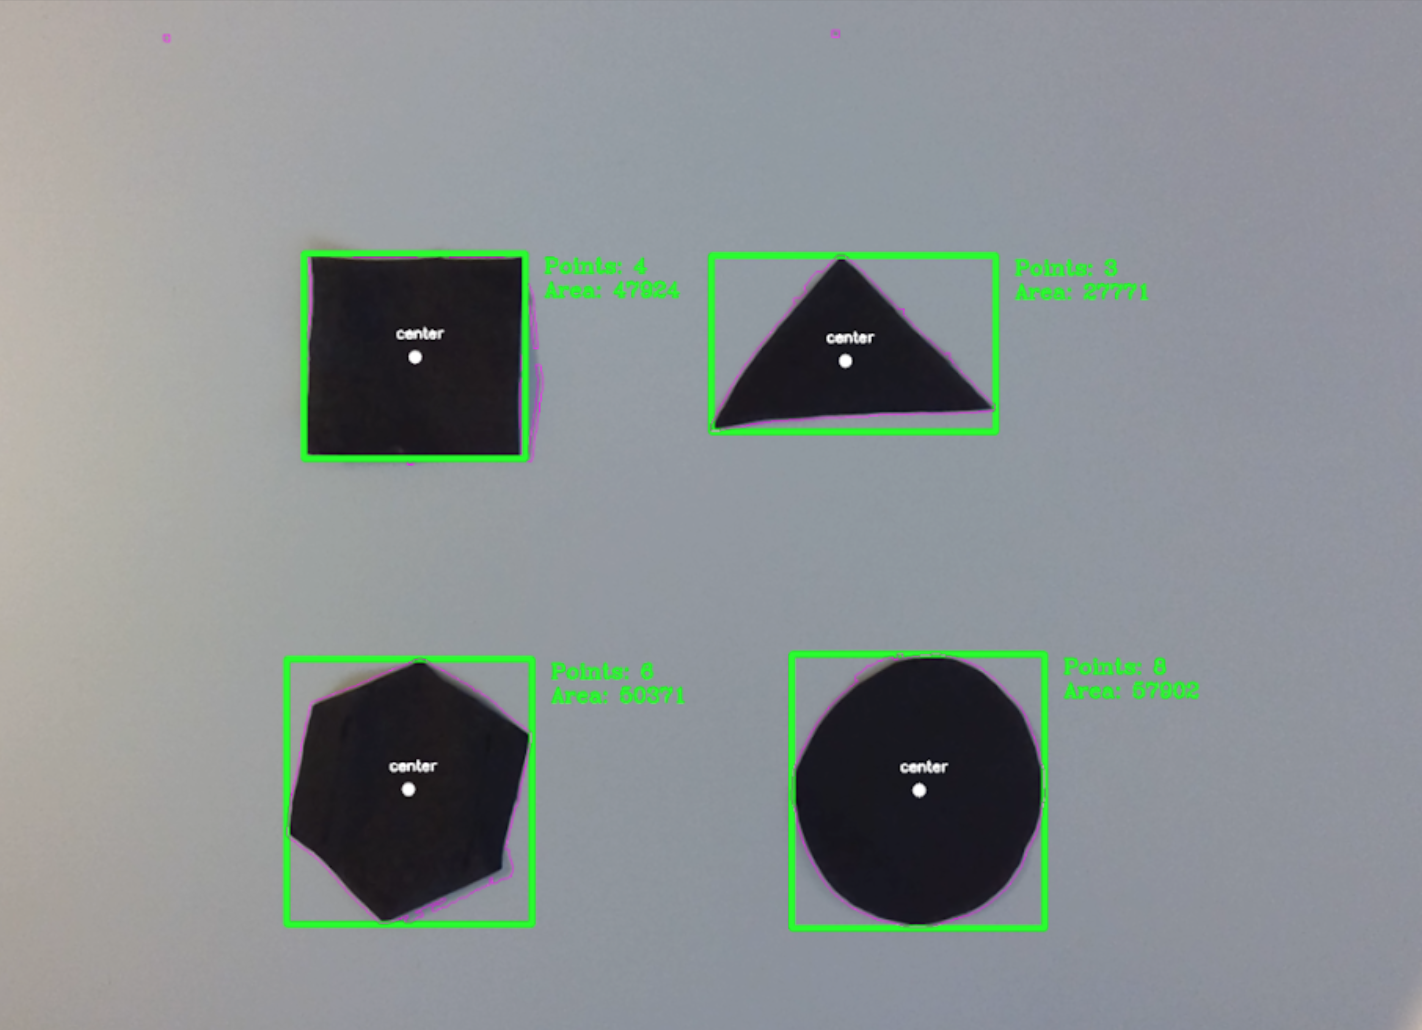
\includegraphics[width=.8\linewidth]{images/objektene.png}
        \caption{Her vises det hvordan programmet detekterer og gjenkjenner objektene som er i kameraet}
        \label{resulat:objekt}
    \end{figure}

    
\section{Diskusjon}
    \subsection{Simulering og test i RobotStudio}
        Tekststrengen som ble sendt fra Python-programmet ble i første omgang kun lest i sin helhet av programmet i RobotStudio. Når den ble mottatt av programmet i RobotStudio viste seg derimot at det var en utfordring med at Python-programmet sendte samme tekststreng gjentatte ganger. Dette førte til at robotarmen prøvde å hente samme figur flere ganger selv om den allerede var flyttet. 
        
        Løsningen på problemet var å sende tekststrengen inn i en rekke if-setninger. If-setningene sjekket om ny tekststreng var lik den forrige tekststrengen. De sjekket også om x-koordinatene var lik forrige x-koordinat eller om y-koordinatene var lik forrige y-koordinat. Hvis en av tilfellene var sant skulle programmet i RobotStudio se bort i fra denne tekststrengen og vente på neste tekststreng.

        En kombinasjon av at kameraet ikke var montert vinkelrett på arbeidsområdet og at lyset i rommet var dynamisk endrende, kunne skyggene til objektene noen ganger plukkes opp som egne kanter. Dette resulterte i at en trekant noen ganger ble registrert som en firkant og at sirklene ikke ble detektert i det hele tatt. Dette kunne utbedres noe ved å justere på parametrene for sensitivitet i Python programkoden.
        
        På grunn av at kameraet modellerer virkeligheten med piksler var det ikke til å komme unna at en sirkel som ideelt ikke har kanter faktisk får kanter. Med dette kameraets oppløsning ble åtte kanter registrert som en sirkel. Sirkel-problematikken er løst ved å tillate rom for avvik slik at antall kanter for en sirkel kunne være større enn syv, men mindre enn ti. Det måtte også settes en øvre grense slik at ikke alt på arbeidsområde kunne tolkes som en sirkel. 

        OpenCV støtter hovedsakelig bare plug-and-play enheter, noe som skapte problemer for kommunikasjon mellom OpenCV og kameraet. Det viste seg at kameraet hadde flere sensorer som ble knyttet sammen gjennom kamera driveren og programvaren, noe OpenCV ikke klarte å gjøre. Synsvinkelen til kameraet ble derfor noe dårligere enn ønsket. Bildet fra kameraet var også speilvendt som gjorde ting vanskelig da OpenCV behandler dataen med utgangspunkt i det øverste venstre hjørnet. Det var derfor nødvendig å speilvende tilbake bildet før bildeprosesseringen kunne anvendes.

        Speilvendingen av bildet viste seg å være veldig prosesskrevende som resulterte i en treg videostrøm for bildeprosesseringen. En løsning på dette kunne vært å bruke en datamaskin med en kraftigere grafikkprosessor til å håndtere bildeprosesseringen. 

    \subsection{Test med ABB-robotarm}
        Som følge av gjentatte tester med ABB-robotarmen viste det seg at Python programmet detekterte selve robotarmen som en figur og prøvde å sortere denne. Det ble derfor nødvendig å legge inn en pauseposisjon for robotarmen utenfor synet til kameraet, slik at python programmet kunne hente ny posisjon til neste geometriske figur som skulle sorteres.

        Det viste seg ganske fort at trekant figuren som var laget fungerte dårlig. Den var for liten og ujevn i kantene. Noen ganger ble den registrert som en annen geometrisk figur og robotarmen prøvde å sortere den til en annen endestasjon enn for trekanter. Det viste seg også at størrelsen på trekanten gjorde det vanskelig for sugekoppen å få tak i den. Derfor ble etterhvert trekanten ekskludert fra gjennomføringen av prosjektet. 

        Mellom hver test i ARIS-laben viste det seg at kameraet i taket hadde flyttet seg litt. Dette medførte at arbeidsområdet til ABB-robotarmen også hadde flyttet seg. Det var derfor nødvendig med en justering av arbeidsområdet før det var mulig å kjøre programmet. Det hadde vært ønskelig med et kamera som var bedre montert i taket og som står vinkelrett mot basen til robotarmen.

    \subsection{Forslag til forbedring av prosjektet}
        I dette prosjektet ble det brukt et 2D kamera festet i taket over arbeidsområdet. Dette begrenset synsvinkelen til kun å oppfatte hvor objektene lå i xy-planet. Det var dog ikke mulig å oppfatte høyden på objektene. En utbedring på dette kunne blant annet ha vært å montere et ekstra kamera som hadde kunnet oppfatte høyden på objektene slik at høyden ikke hadde måttet forhåndsdefineres. 

        For objektgjenkjenning kunne det alternativt blitt trent opp en modell til å gjenkjenne figurene i stedet for å gjenkjenne antall kanter. Dette hadde resultert i en mer nøyaktig bildegjenkjenning hvor flere objekter kunne blitt implementert, men det hadde samtidig krevd flere arbeidstimer noe det ikke var tilstrekkelig mange av i dette prosjektet.  

        For å øke bildefrekvensen kunne det blitt benyttet en kraftigere datamaskin. Dette ville forbedret nøyaktigheten og samtidig fikset mange av problemene som oppstod underveis, f.eks. utfordringen ved at Python programmet sendte samme informasjons-streng flere ganger

    
\section{Konklusjon}
    Det ble lagt mye tid i undersøkelser rundt det første prosjektet som ble igangsatt: finne riktig bibliotek, nøkkelkode til Choreographe, dokumentasjon om NAO osv. Prosjektet var kommet godt i gang da roboten ble ødelagt. Etter en god idemyldring var det mulig å omstille seg og finne et prosjekt som beholdt samme grunntanke. Dette ga en myk overgang til prosjekt nummer to.

    OpenCV viste seg å være et meget godt verktøy å bruke for nykommere i bildeprosessering og kunstig intelligens. Emnet \textit{ELVE3610 Robotteknikk} har gitt innføring i å lage funksjoner i Python, samt bli kjent med hvordan funksjoner ser ut. Dette ga en bedre forutsetning til å tolke funksjonene i OpenCV-biblioteket og vite hvordan å utnytte disse. Hadde prosjektperioden vært lenger eller  hadde det vært mulig å trene en egen maskinlæringsmodell til å kjenne igjen de geometriske figurene i steden for å bruke kantdeteksjon, kanskje til og med laget egenspesifiserte figurer den kjente igjen. 

    En av laboratorieoppgavene i kurset innebar å bruke socket programmering som et kommunikasjonsledd mellom roboten og en ekstern datamaskin ved hjelp av funksjoner i RAPID (RobotStudio) og et Python-program. Dette konseptet ble godt implementert i prosjektet og gjorde det mulig å kombinere KI med ABB-robotarmen. 

    I arbeidet med programmeringen i RobotStudio hadde prosjektgruppen mye god kunnskap som var opparbeidet gjennom laboratorieoppgavene i faget. Likevel gikk det mye tid til å sette sammen programmodulene og få programmet til å kommunisere på en god måte med Python-programmet. Ved testing viste seg at den virtuelle verden og den virkelige verden ikke alltid er lik. Det var derfor nødvendig med noe finjustering. Dette kom spesielt godt frem ved synkronisering av kameraets arbeidsområde til robotarmens arbeidsområde. 


% trigger a \newpage just before the given reference
% number - used to balance the columns on the last page
% adjust value as needed - may need to be readjusted if
% the document is modified later
%\IEEEtriggeratref{8}
% The "triggered" command can be changed if desired:
%\IEEEtriggercmd{\enlargethispage{-5in}}

% references section

% can use a bibliography generated by BibTeX as a .bbl file
% BibTeX documentation can be easily obtained at:
% http://www.ctan.org/tex-archive/biblio/bibtex/contrib/doc/
% The IEEEtran BibTeX style support page is at:
% http://www.michaelshell.org/tex/ieeetran/bibtex/
%\bibliographystyle{IEEEtran}
% argument is your BibTeX string definitions and bibliography database(s)
%\bibliography{IEEEabrv,../bib/paper}
%
% <OR> manually copy in the resultant .bbl file
% set second argument of \begin to the number of references
% (used to reserve space for the reference number labels box)

% Referanse listen
\bibliography{Robtek_referanser}
\bibliographystyle{ieeetr}

\onecolumn % Make appendices single column
\newpage
\appendices
\section{NAO}
\subsection{NAO - kode}
NAO snakker og går
\lstinputlisting[language=Python,firstline=2]{../NAOProsjekt/NAO20.py}
NAO lokaliserer en rød ball og går til den
\lstinputlisting[language=Python,firstline=14]{../NAOProsjekt/NAOtesting.py}

\section{ABB}
\subsection{Utstyrsliste}
\begin{figure}[!htb]
    \centering
    \textbf{Software}\par\medskip 
    \begin{tabular}{|l|l|}
        \hline
        \textbf{Program} & \textbf{Type}\\
        \hline
        RobotStudio (RAPID) & Programmeringsmiljø\\
        \hline
        Python & Programmeringsspråk \\
        \hline
        OpenCV & Bibliotek \\
        \hline
        socket & Bibliotek \\
        \hline
    \end{tabular}
    \label{app:soft}
\end{figure}
\begin{figure}[!htb]
    \centering
    \textbf{Hardware}\par\medskip 
    \begin{tabular}{|l|l|l|}
        \hline
        \textbf{Utstyr} & \textbf{Type} & \textbf{Fabrikant}\\
        \hline
        Robotarm & IRB 140, 6kg, 0.81m & ABB\\
        \hline
        Kamera & UI-3360CP & iDS\\
        \hline
        Datamaskin & Laptop & Windows \\
        \hline
        FlexPendant & Kontroller & ABB \\
        \hline
        Sugekopp & Verktøy til robotarm &  \\
        \hline
    \end{tabular}
    \label{app:hard}
\end{figure}

\subsection{ABB - kode}
Objektgjenkjenning
\lstinputlisting[language=Python, firstline=3, lastline=158]{../ABB_Prosjekt/center_contour.py}
Klient koden
\lstinputlisting[language=Python, firstline=3]{../ABB_Prosjekt/Client_ABB.py}
% that's all folks
\end{document}